
\begin{figure}
\centering

\begin{subfigure}[b]{0.75\textwidth}
    \centering
    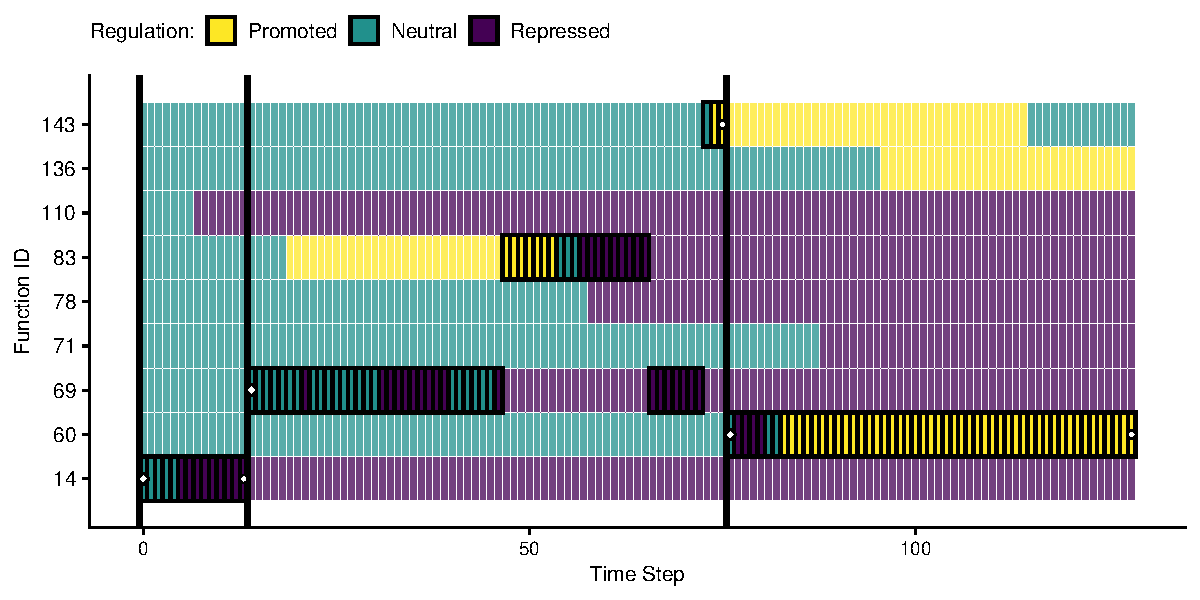
\includegraphics[width=\textwidth]{chapters/05-tag-based-genetic-regulation/media/boolean-calc-prefix-networks/case-study-trace-id-24400-test_id-420-regulator-state-horizontal.pdf}
    \caption{\small  Module regulation over time for a NAND operation.}
    \label{chapter:tag-based-regulation:subfig:bc-nand-exec-trace}
\end{subfigure}%

\begin{subfigure}[b]{0.5\textwidth}
    \centering
    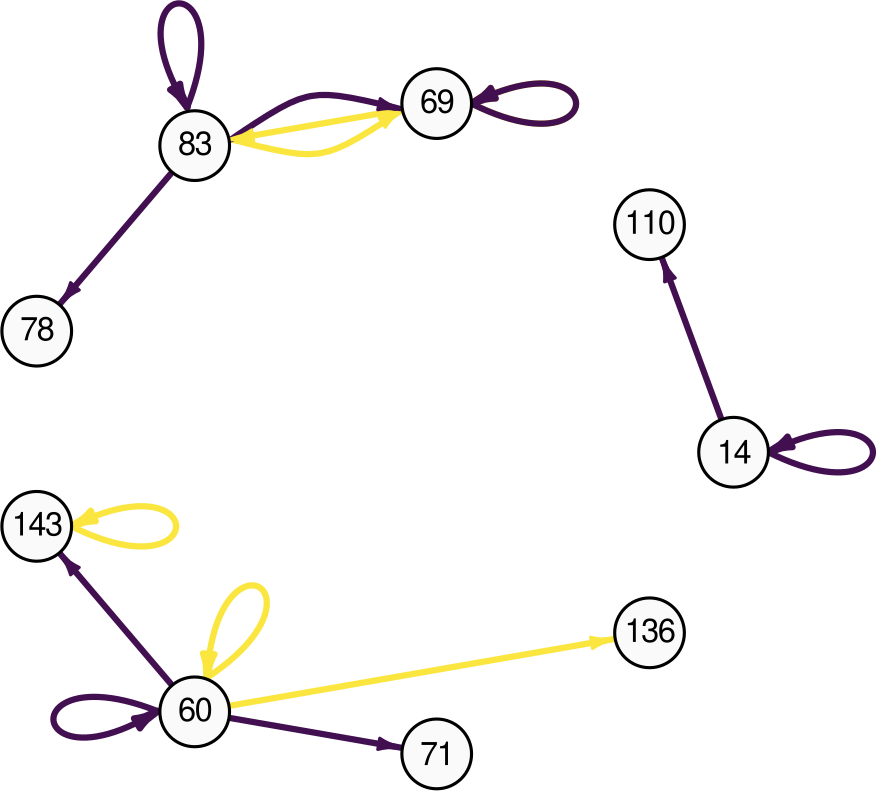
\includegraphics[width=0.6\textwidth]{chapters/05-tag-based-genetic-regulation/media/boolean-calc-prefix-networks/case-study-id-24400-test-420-network-cropped.png}
    \caption{\small NAND regulatory network.}
    \label{chapter:tag-based-regulation:subfig:bc-nand-reg-network}
\end{subfigure}%
\hfill
\begin{subfigure}[b]{0.5\textwidth}
    \centering
    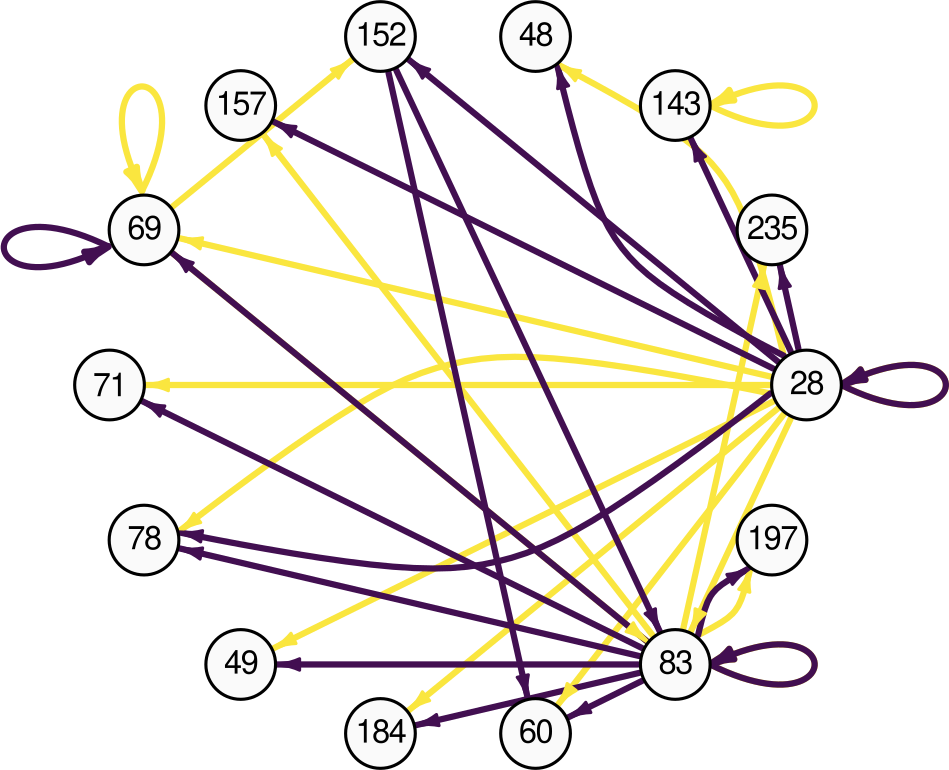
\includegraphics[width=0.6\textwidth]{chapters/05-tag-based-genetic-regulation/media/boolean-calc-prefix-networks/case-study-id-24400-test-134-network-cropped.png}
    \caption{\small NOR regulatory network.}
    \label{chapter:tag-based-regulation:subfig:bc-nor-reg-network}
\end{subfigure}%

\begin{subfigure}[b]{0.75\textwidth}
    \centering
    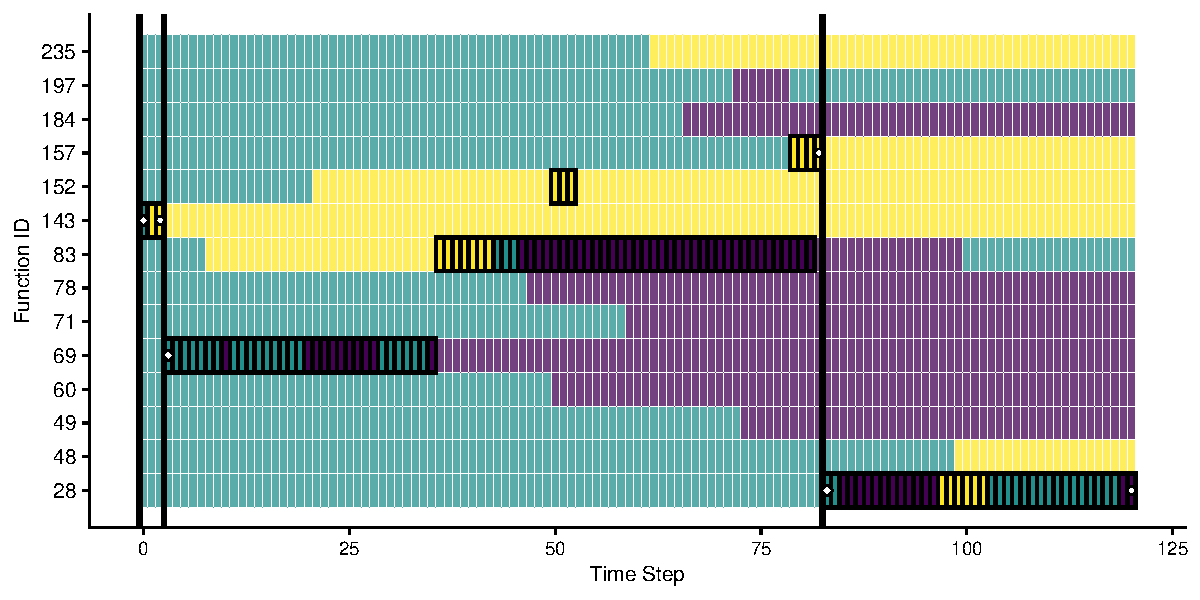
\includegraphics[width=0.95\textwidth]{chapters/05-tag-based-genetic-regulation/media/boolean-calc-prefix-networks/case-study-trace-id-24400-test_id-134-regulator-state-horizontal-nolegend.pdf}
    \caption{\small Module regulation over time for a NOR operation.}
    \label{chapter:tag-based-regulation:subfig:bc-nor-exec-trace}
\end{subfigure}%

\caption{\small 
\textbf{Execution traces of a successful SignalGP program computing a NAND operation (a) and a NOR operation (d).}
(b) and (c) show the directed graphs representing the regulatory networks associated with traces (a) and (d), respectively.
These visualizations are in the same format as those in Figure \ref{chapter:tag-based-regulation:fig:signal-counting-example-networks}.}
\label{chapter:tag-based-regulation:fig:boolean-calc-prefix-example-networks}
\end{figure}
